\documentclass[]{article}

% Imported Packages
%------------------------------------------------------------------------------
\usepackage{amssymb}
\usepackage{amstext}
\usepackage{amsthm}
\usepackage{amsmath}
\usepackage{enumerate}
\usepackage{fancyhdr}
\usepackage[margin=1in]{geometry}
\usepackage{graphicx}
\usepackage{extarrows}
\usepackage{setspace}
\usepackage{float}
\usepackage{vhistory}
%------------------------------------------------------------------------------

% Header and Footer
%------------------------------------------------------------------------------
\pagestyle{plain}  
\renewcommand\headrulewidth{0.4pt}                                      
\renewcommand\footrulewidth{0.4pt}                                    
%------------------------------------------------------------------------------

% Title Details
%------------------------------------------------------------------------------
\title{Deliverable \#3 Template}
\author{SE 3A04: Software Design II -- Large System Design}
\date{}                               
%------------------------------------------------------------------------------

% Document
%------------------------------------------------------------------------------
\begin{document}

\maketitle	

\section{Introduction}
\label{sec:introduction}
% Begin Section

This section should provide an brief overview of the entire document.

\subsection{Purpose}
\label{sub:purpose}
% Begin SubSection
\begin{enumerate}[a)]
	\item Delineate the purpose of the document
	\item Specify the intended audience for the document
\end{enumerate}
% End SubSection

\subsection{System Description}
\label{sub:system_description}
% Begin SubSection
\begin{enumerate}[a)]
	\item Give a brief description of the system. This could be a paragraph or two to give some context to this document.
\end{enumerate}
% End SubSection

\subsection{Overview}
\label{sub:overview}
% Begin SubSection
\begin{enumerate}[a)]
	\item Describe what the rest of the document contains 
	\item Explain how the document is organised
\end{enumerate}

% End SubSection

% End Section

\section{State Charts for Controller Classes}
\label{sec:state_charts_for_controller_classes}

\begin{figure}[H]
	\centering
	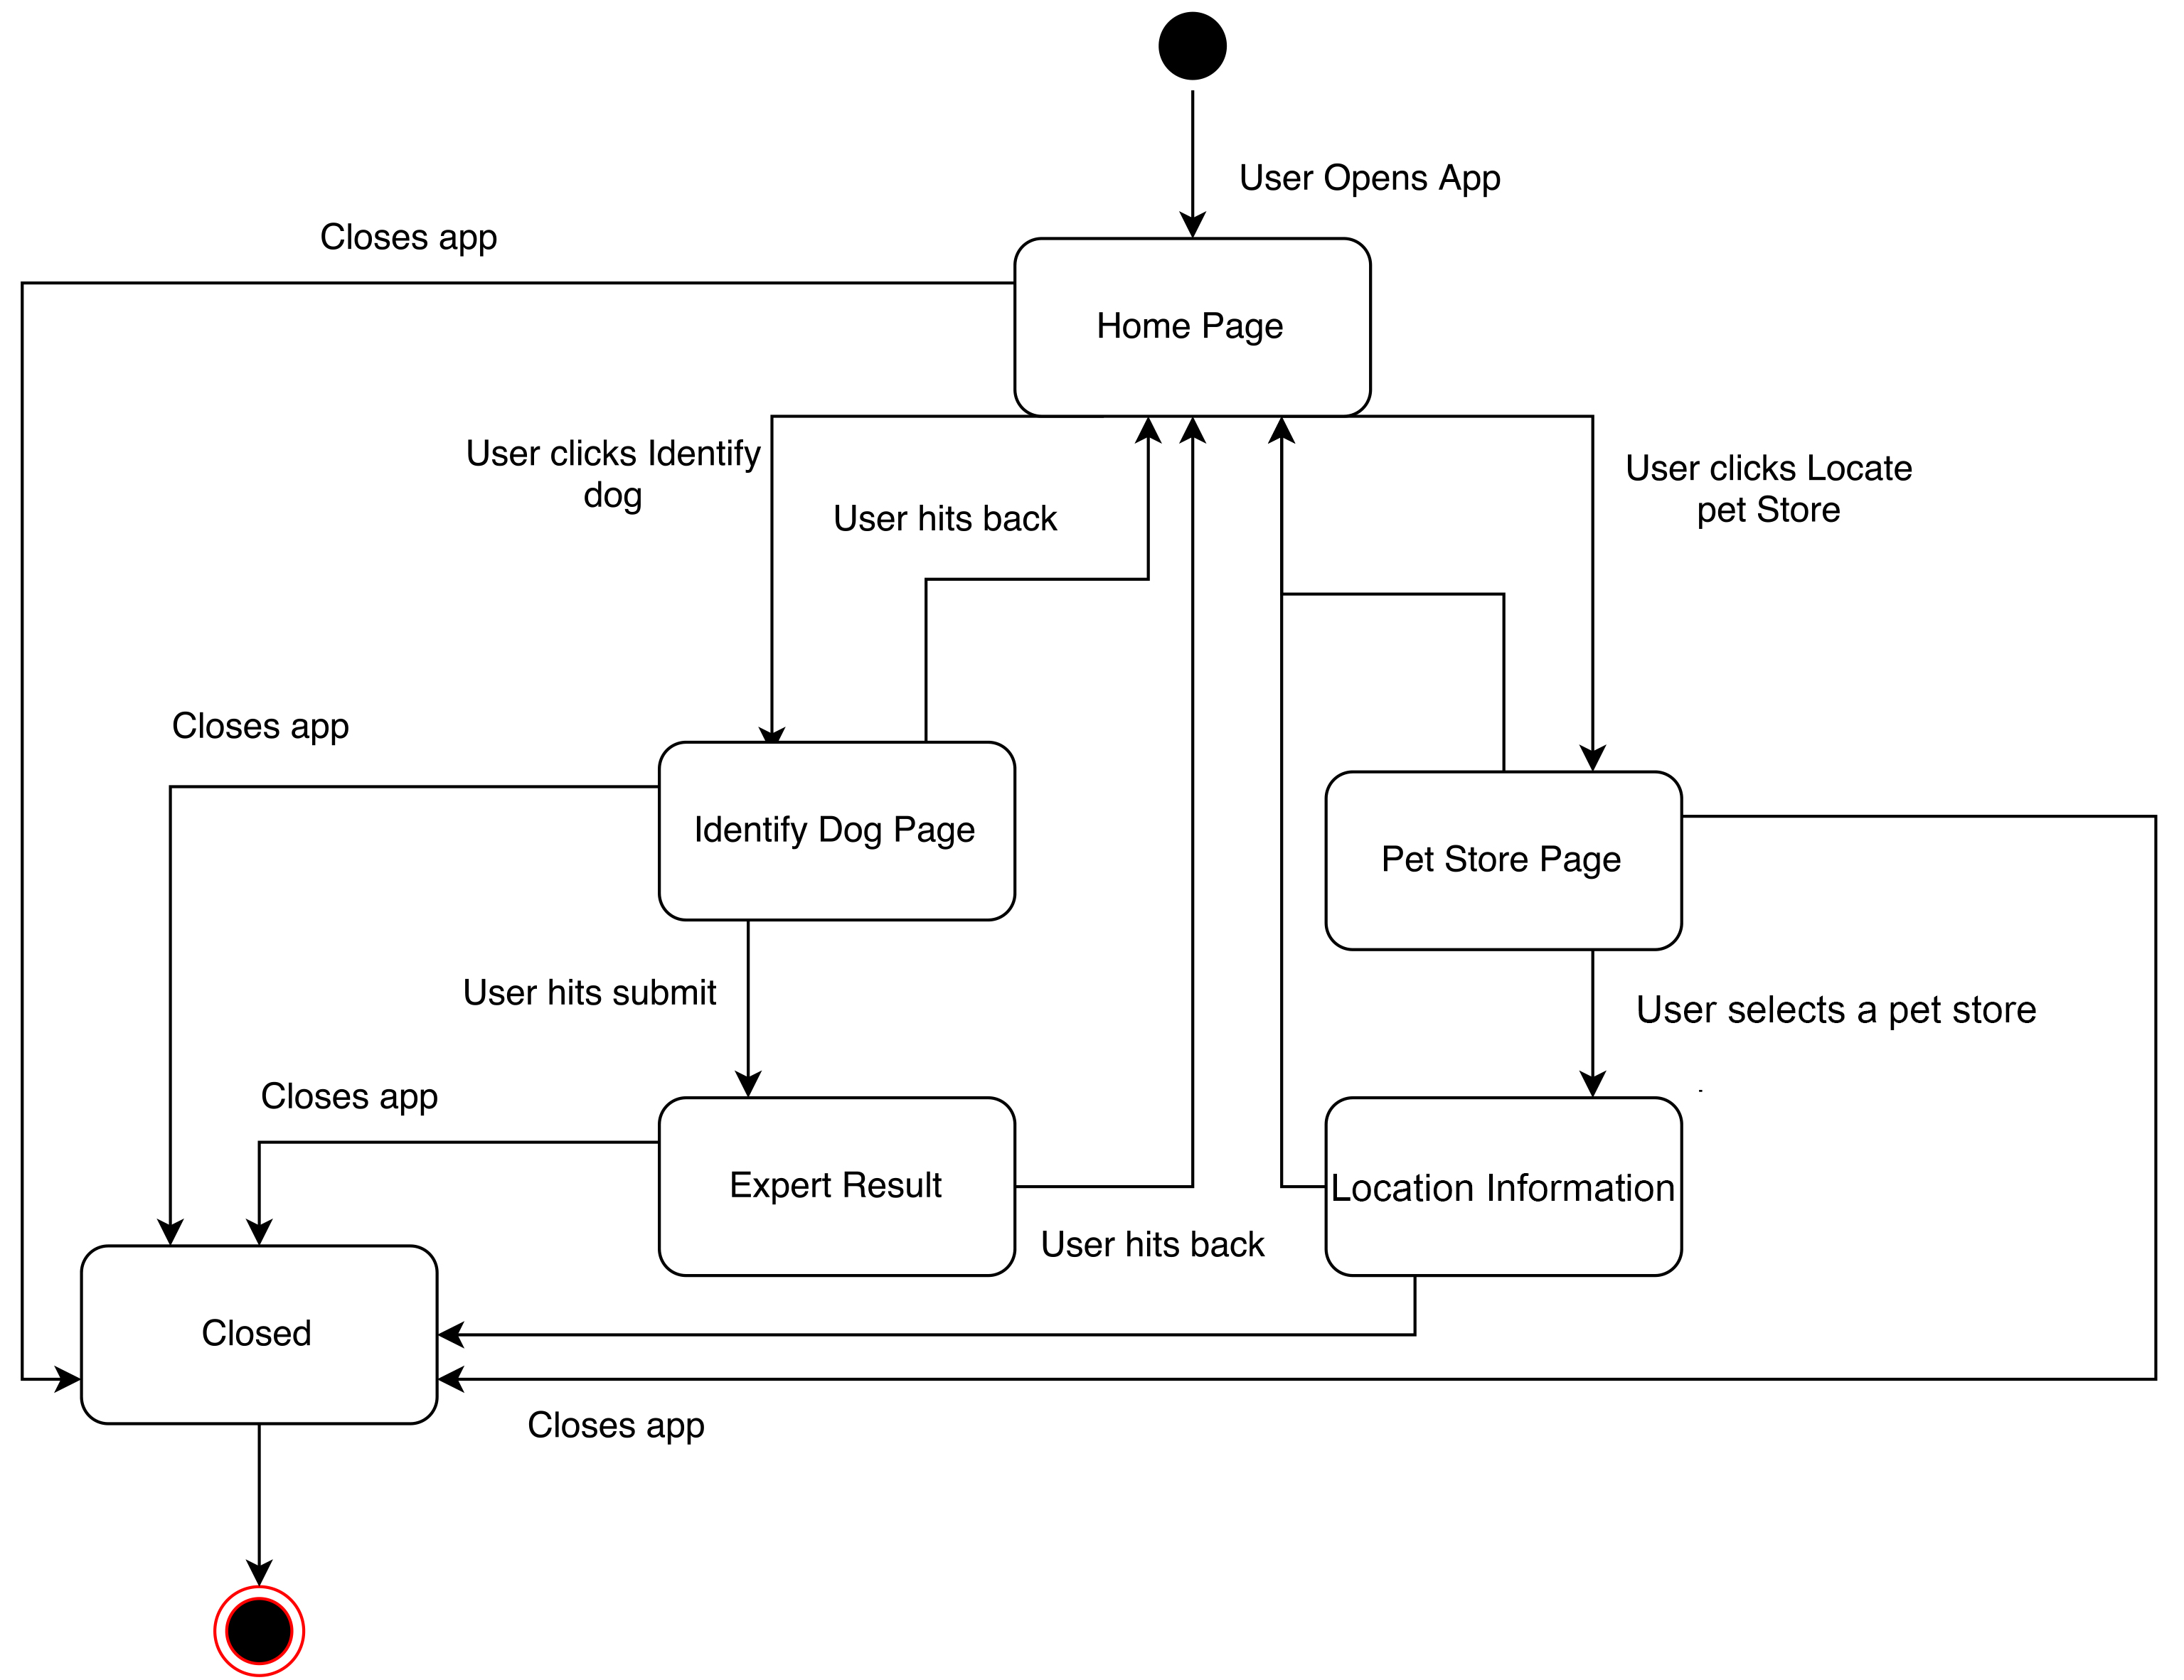
\includegraphics[width=\textwidth]{ForumController.jpg}
	\caption{\label{fig:analysisclassdiagram}The state chart of the Forum Controller of the WhoDatDog system.}
\end{figure}

\begin{figure}[H]
	\centering
	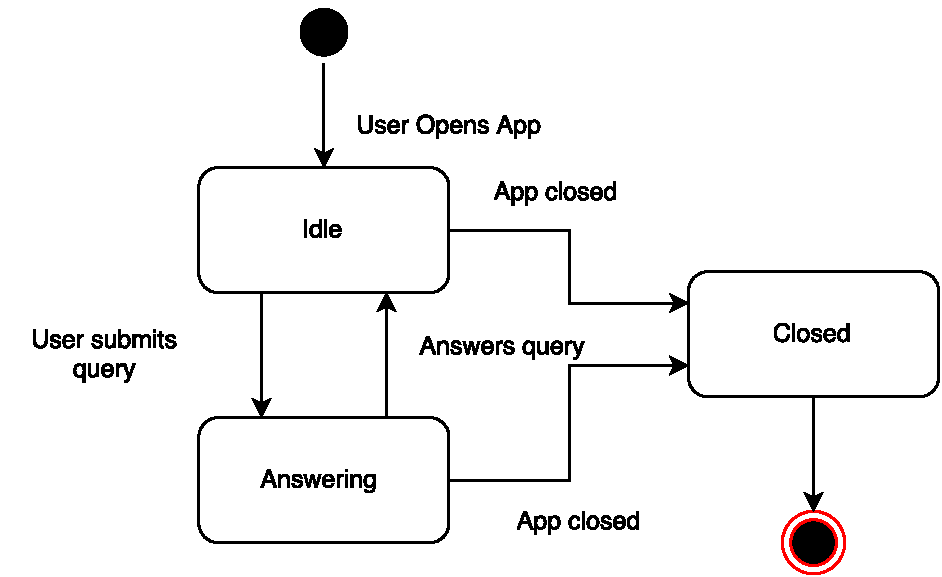
\includegraphics[width=\textwidth]{ExpertController.pdf}
	\caption{\label{fig:analysisclassdiagram}The state chart of the Expert Controller of the WhoDatDog system.}
\end{figure}

There will be at least  5 Expert Controller but they will have the same state chart



\begin{figure}[H]
	\centering
	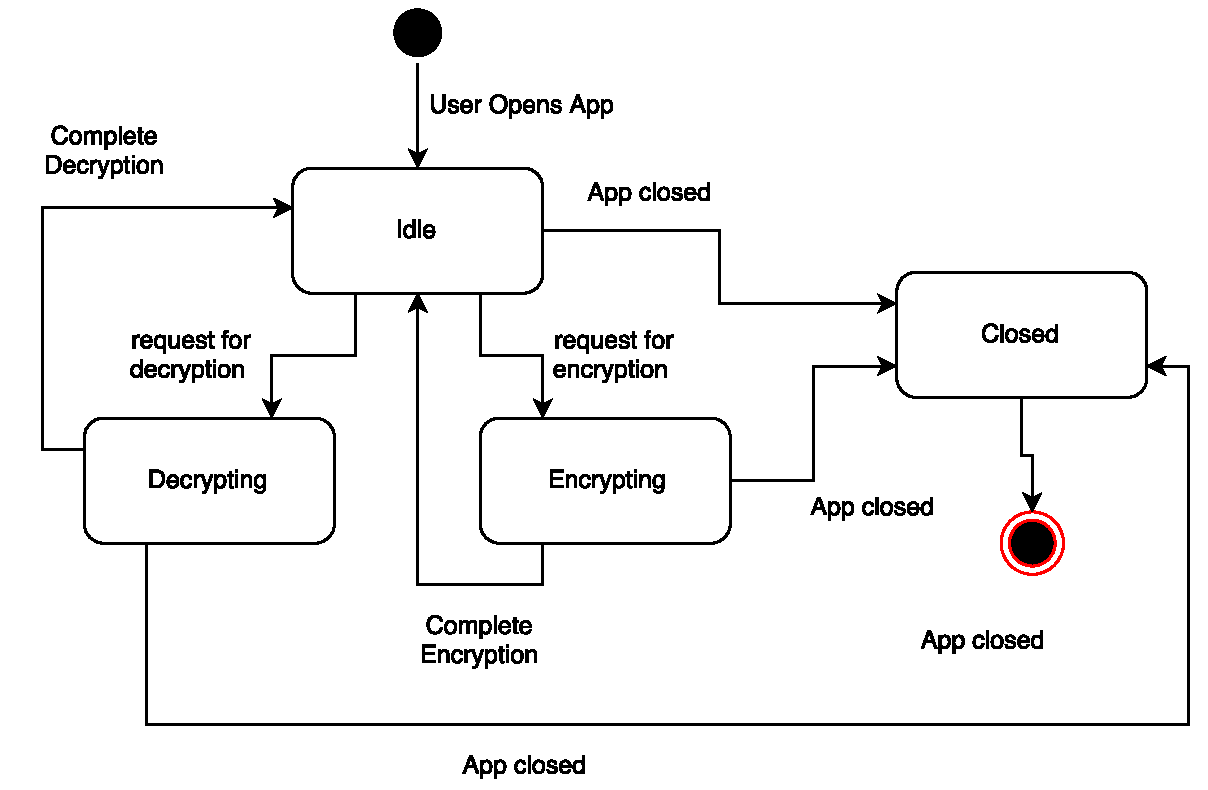
\includegraphics[width=\textwidth]{EncryptionController.pdf}
	\caption{\label{fig:analysisclassdiagram}The state chart of the Encryption Controller of the WhoDatDog system.}
\end{figure}


\begin{figure}[H]
	\centering
	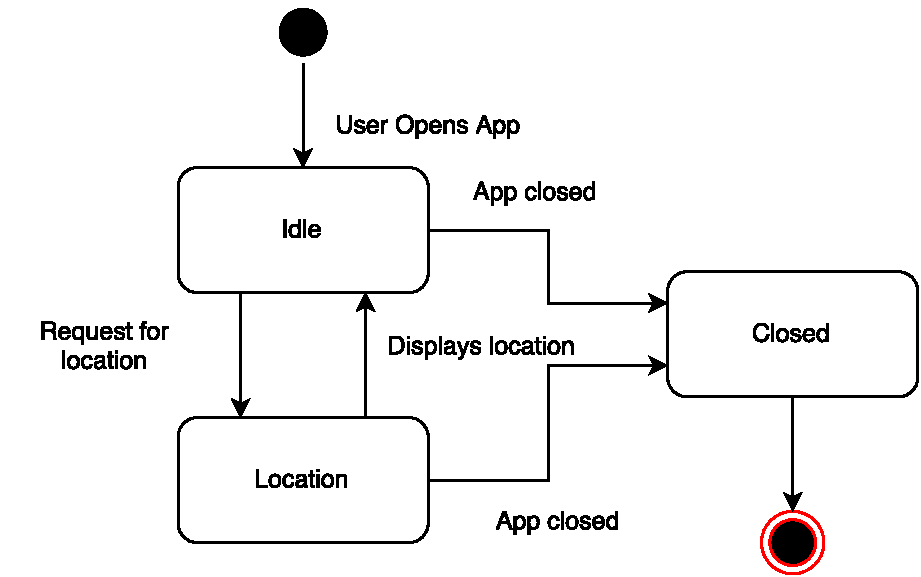
\includegraphics[width=\textwidth]{GoogleMapsController.pdf}
	\caption{\label{fig:analysisclassdiagram}The state chart of the Google Maps Controller of the WhoDatDog system.}
\end{figure}


\begin{figure}[H]
	\centering
	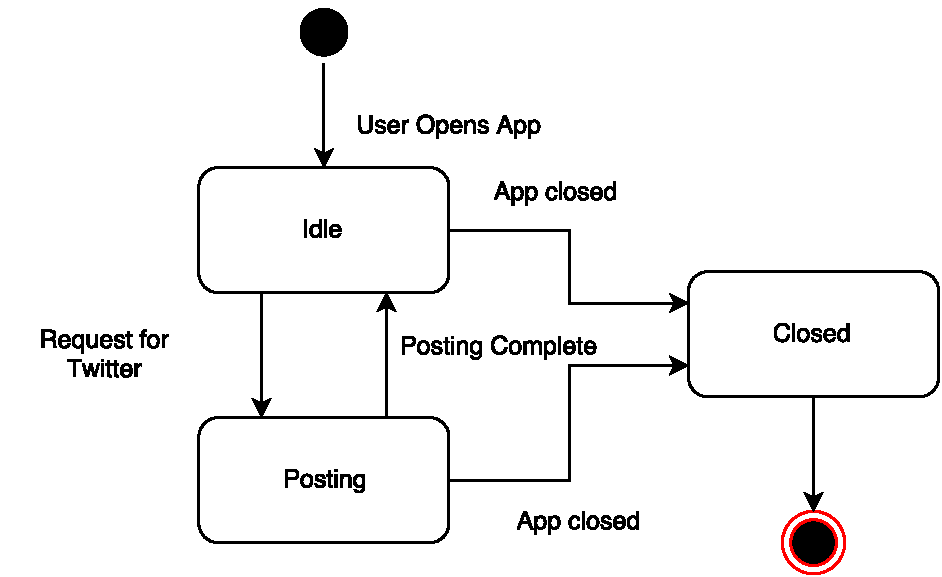
\includegraphics[width=\textwidth]{TwitterController.pdf}
	\caption{\label{fig:analysisclassdiagram}The state chart of the Twitter Controller of the WhoDatDog system.}
\end{figure}




\section{Sequence Diagrams}
\label{sec:sequence_diagrams}
\begin{figure}[H]
	\centering
	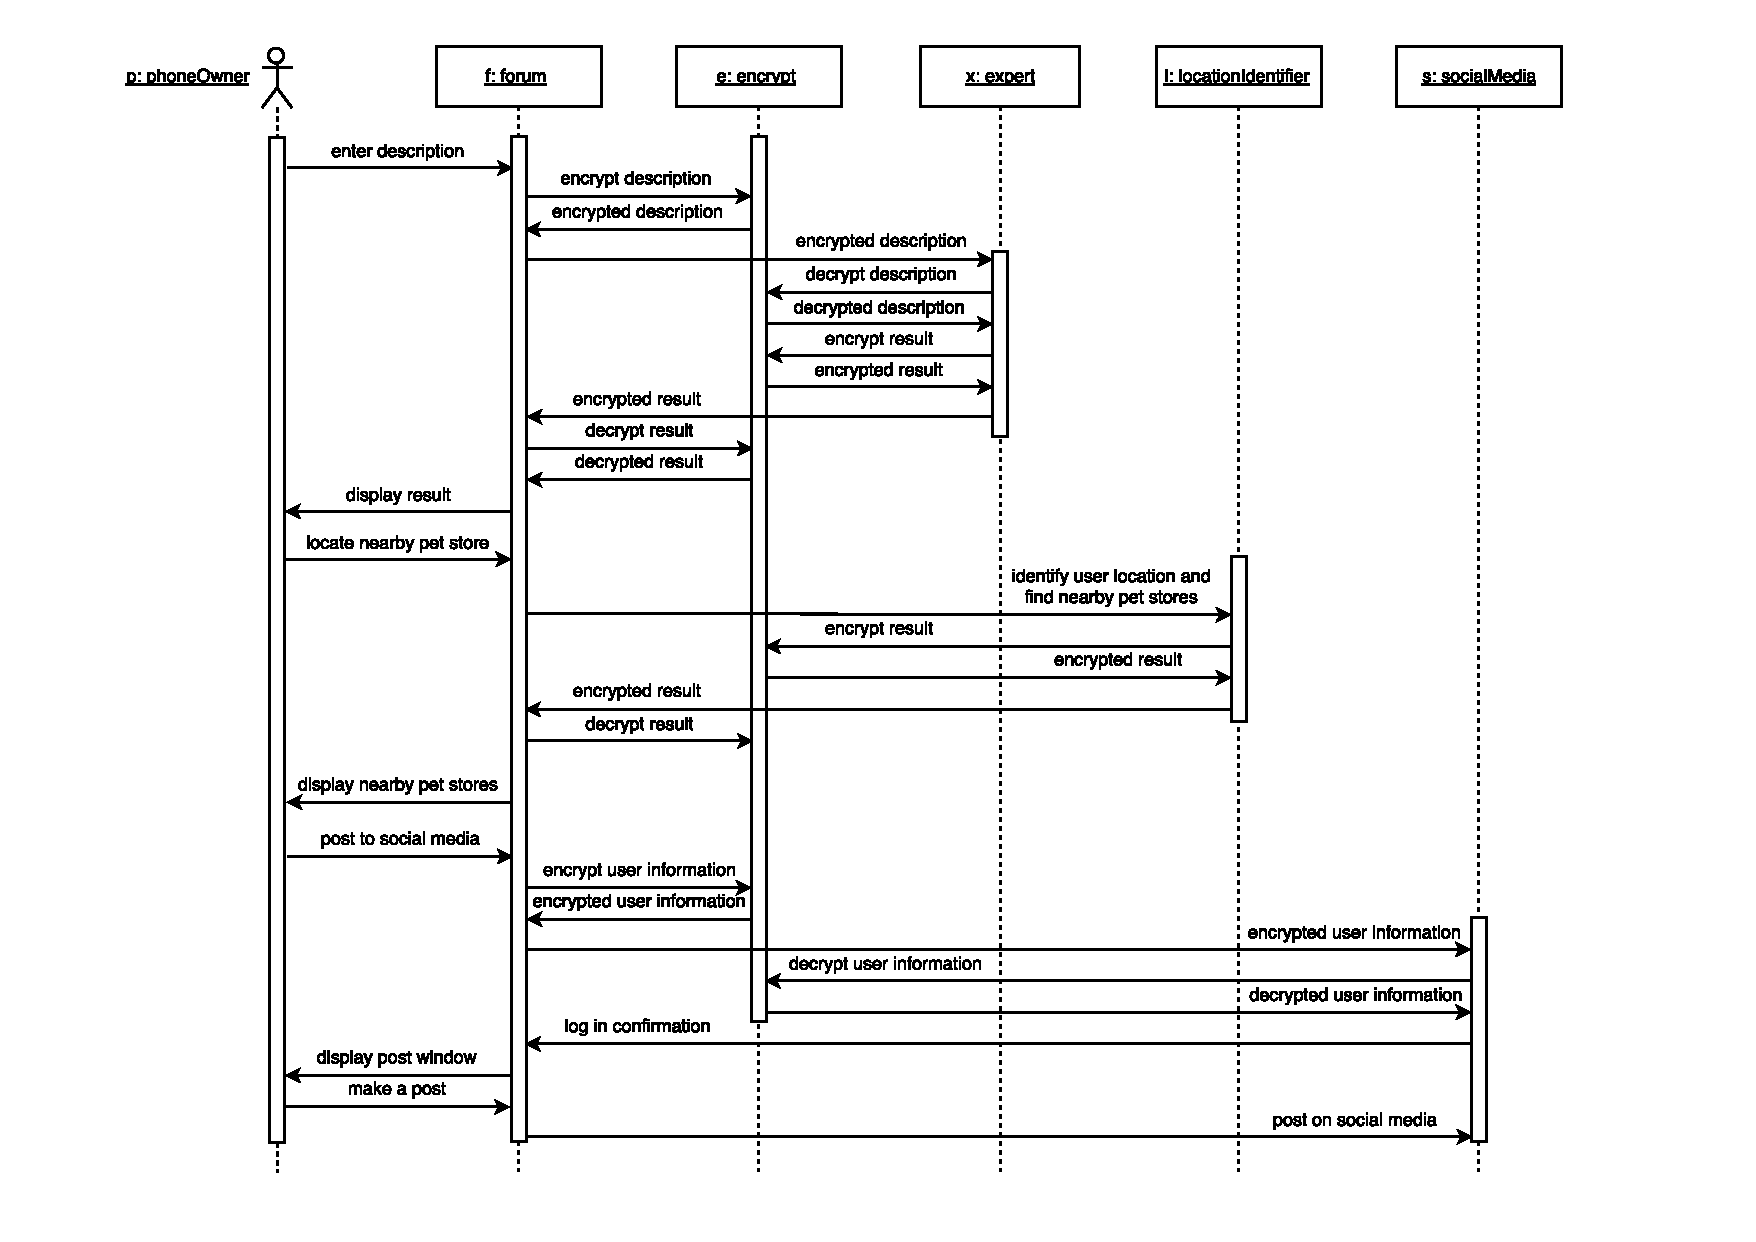
\includegraphics[width=\textwidth]{sequencediagram.pdf}
	\caption{\label{fig:analysisclassdiagram}The sequence diagram of the WhoDatDog system.}
\end{figure}

\section{Detailed Class Diagram}

\begin{figure}[H]
	\centering
	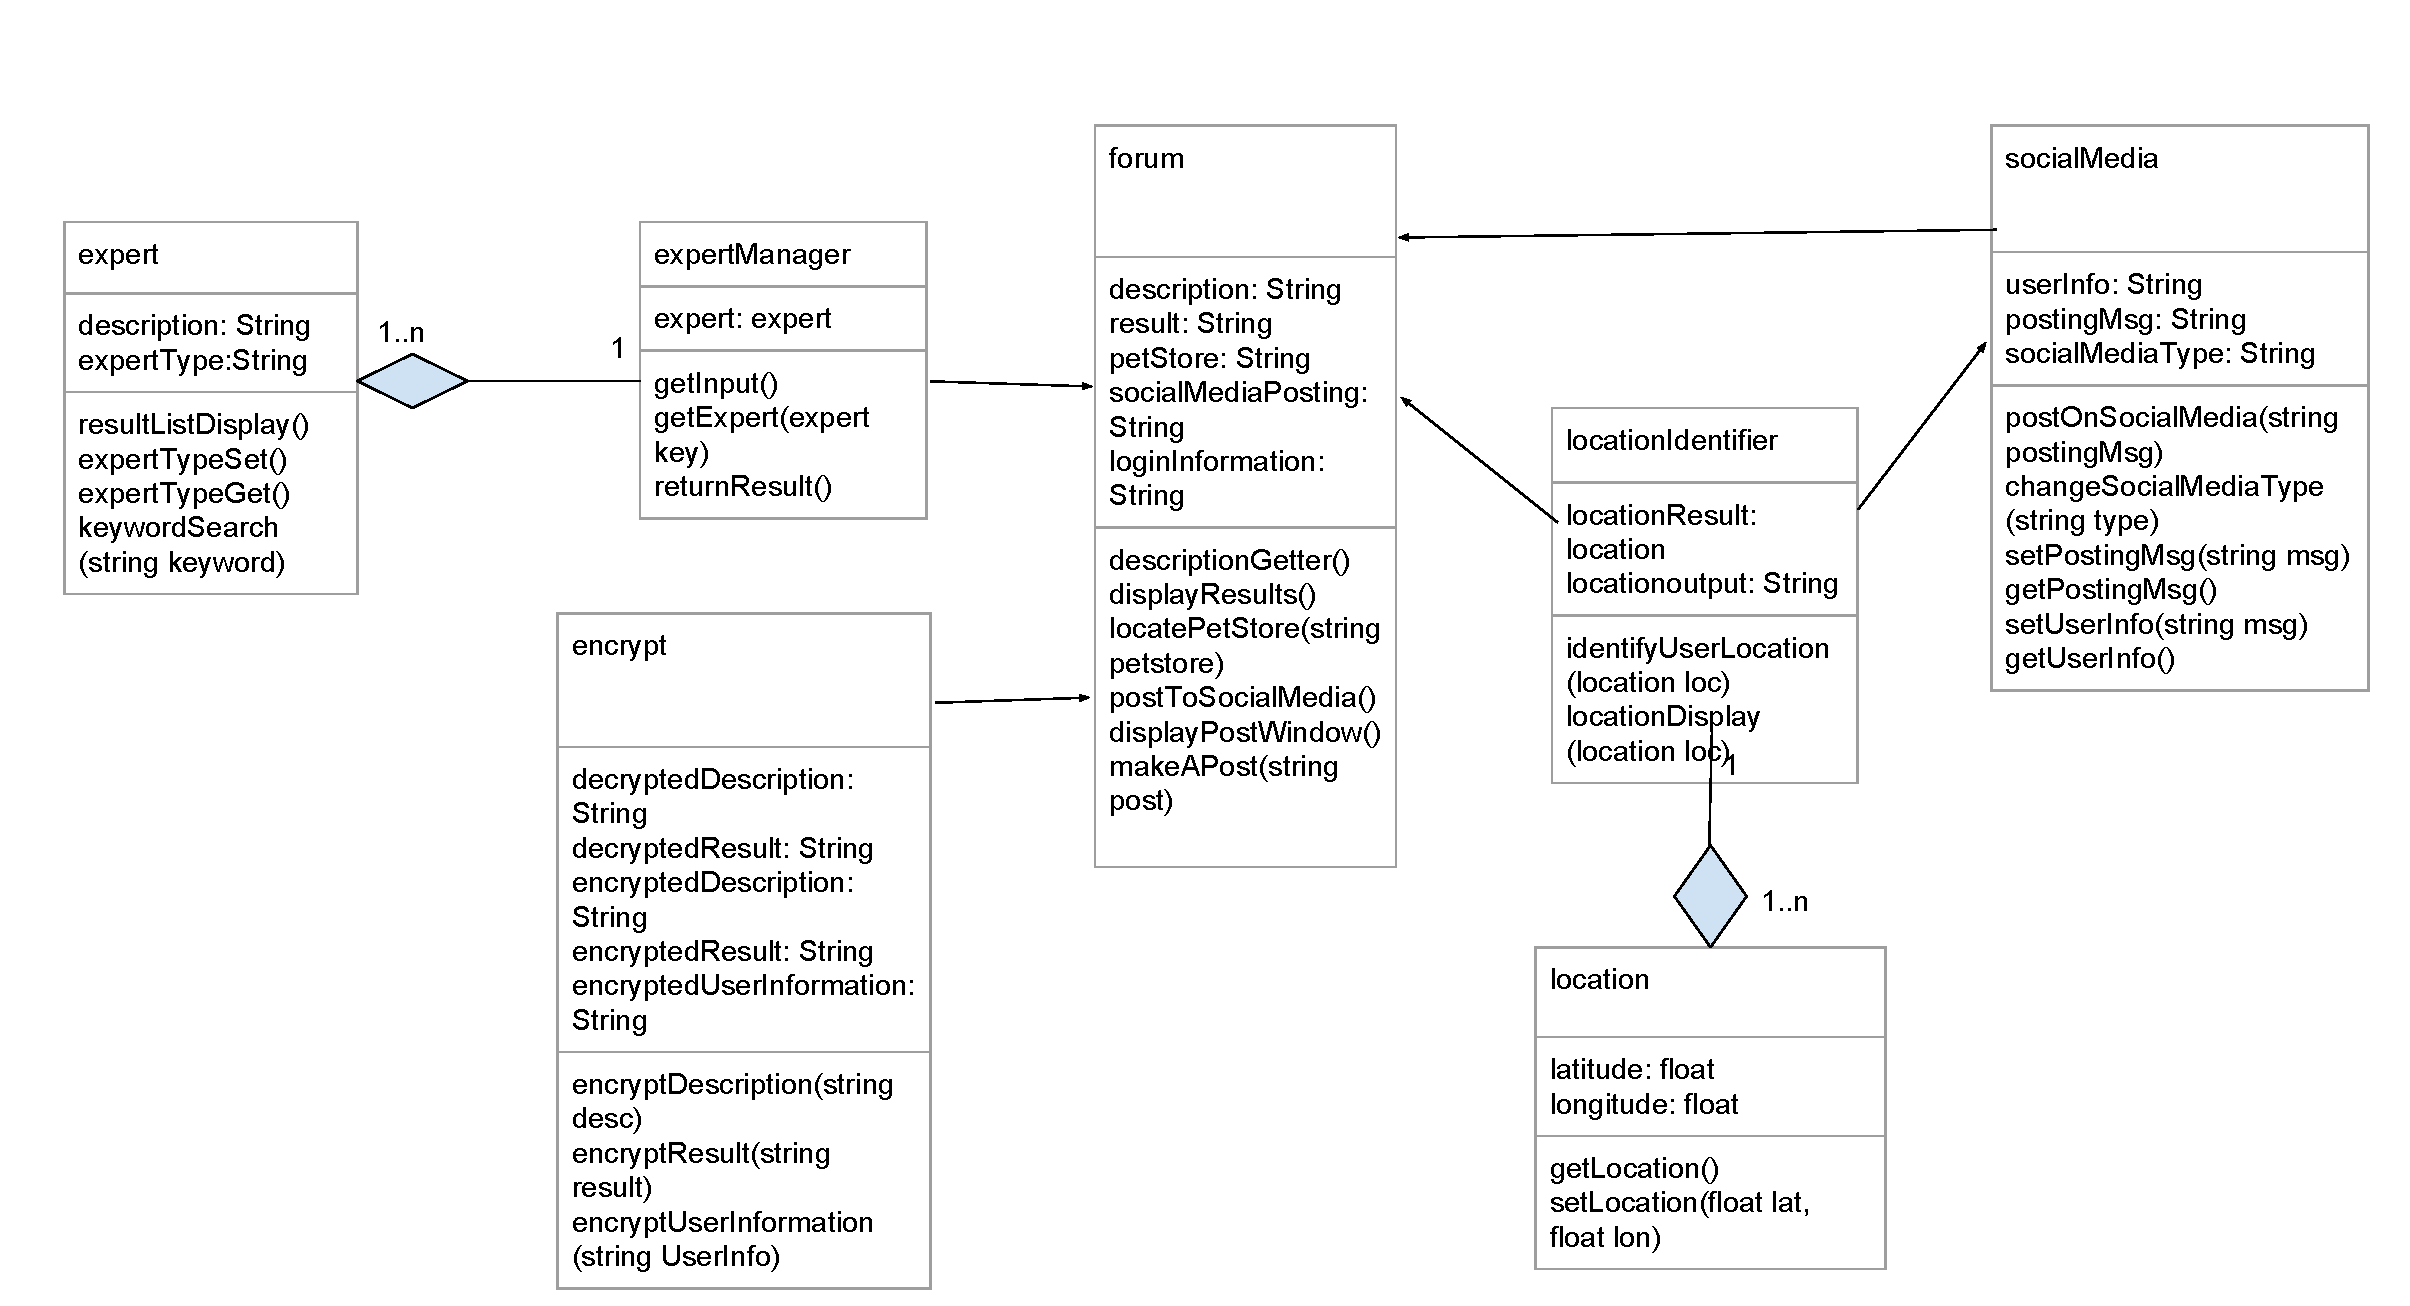
\includegraphics[width=\textwidth]{DetailClassDiagram.pdf}
	\caption{\label{fig:analysisclassdiagram}The Detailed Class diagram of the WhoDatDog system.}
\end{figure}

\appendix
\section{Division of Labour}


test

\newpage
--------------------------------------------------------